\documentclass[12pt, letterpaper]{article}
\usepackage[utf8]{inputenc}
\usepackage[spanish,es-tabla]{babel}
\usepackage{graphicx}
\usepackage{amsmath}
\usepackage{amsfonts}
\usepackage{booktabs}
\usepackage{float}
\usepackage{hyperref}
\usepackage{geometry}
\usepackage{listings}
\usepackage{xcolor}
\usepackage{caption}
\usepackage{subcaption}
\usepackage{fancyhdr}
\usepackage[linesnumbered,ruled,vlined]{algorithm2e}

\geometry{margin=2.5cm}

\hypersetup{
    colorlinks=true,
    linkcolor=blue,
    filecolor=magenta,      
    urlcolor=cyan,
    pdftitle={Reporte Final 3er Parcial},
}

\lstset{
  language=Python,
  basicstyle=\ttfamily\small,
  keywordstyle=\color{blue}\bfseries,
  commentstyle=\color{gray},
  stringstyle=\color{orange},
  numbers=left,
  numberstyle=\tiny,
  breaklines=true,
  frame=single
}

\pagestyle{fancy}
\fancyhf{}
\setlength{\headheight}{15pt}
\fancyhead[L]{\small\textcolor{gray}{Técnicas de Inteligencia Artificial}}
\fancyhead[R]{\small\textcolor{gray}{Proyecto Tercer Parcial}}
\fancyfoot[C]{\thepage}
\renewcommand{\headrulewidth}{0.5pt}

\begin{document}

% ==========================================
% PORTADA
% ==========================================
\begin{titlepage}
    \centering
    \vspace*{1cm}
    
    {\Large\textbf{Benemérita Universidad Autónoma de Puebla}}\\[0.5cm]
    {\large\textbf{Facultad de Ciencias de la Computación}}\\[1.5cm]
    
    {\large\textbf{Materia: Técnicas de Inteligencia Artificial}}\\[1cm]
    
    \rule{\linewidth}{0.5mm} \\[0.5cm]
    {\LARGE\textbf{Ajuste de Hiperparámetros de una RNA mediante Algoritmo Metaheurístico Híbrido GA+GWO}}\\[0.5cm]
    \rule{\linewidth}{0.5mm} \\[2cm]
    
    \textbf{Integrantes del equipo:}\\
    \vspace{0.3cm}
    \textit{Gael Askary Razo Montañez}\\
    \textit{Isaac Aguilar Durán}\\
    \textit{Alejandro Hernández Hernández}\\
    \textit{José Ángel Cambranis Sánchez}\\[1cm]
    
    \textbf{Profesor:}\\
    \vspace{0.1cm}
    \textit{Dr. Iván Olmos Pineda}\\[1cm]
    
    \vfill
    {\large Mayo 2026}
\end{titlepage}

\newpage
\tableofcontents
\vspace{1cm}
\listoffigures
\vspace{1cm}
\listoftables
\newpage

% ==========================================
% SECCIÓN 1: BASE DE DATOS
% ==========================================
\section{Base de Datos}
El conjunto de datos utilizado para la clasificación en este proyecto proviene del archivo acumulativo de observaciones fotométricas de la misión Kepler de la NASA (\textit{NASA Kepler Exoplanet Search Results}).

\subsection{Origen y Propósito}
El dataset fue creado para catalogar y clasificar los objetos de interés de Kepler (KOI, por sus siglas en inglés) que han sido detectados por el telescopio espacial Kepler entre los años 2009 y 2018. El objetivo principal o propósito de aplicar aprendizaje automático sobre este dataset es determinar mediante clasificación multiclase si un evento de tránsito estelar es un exoplaneta confirmado (\texttt{CONFIRMED}), un falso positivo (\texttt{FALSE POSITIVE}), o un candidato no resuelto (\texttt{CANDIDATE}).

\subsection{Descripción de Características}
El dataset final tras el preprocesamiento consta de 41 variables continuas y una clase objetivo. En la Tabla \ref{tab:features} se detallan las variables más representativas.

\begin{table}[H]
    \centering
    \caption{Características Principales del Dataset Kepler}
    \label{tab:features}
    \resizebox{\textwidth}{!}{
    \begin{tabular}{@{}lll@{}}
        \toprule
        \textbf{Atributo} & \textbf{Tipo} & \textbf{Descripción} \\ \midrule
        \texttt{koi\_period} & Continuo & Período orbital del tránsito (días). \\
        \texttt{koi\_impact} & Continuo & Parámetro de impacto del tránsito estelar. \\
        \texttt{koi\_duration} & Continuo & Duración del tránsito (horas). \\
        \texttt{koi\_depth} & Continuo & Profundidad del tránsito (partes por millón). \\
        \texttt{koi\_prad} & Continuo & Radio planetario estimado (radios terrestres). \\
        \texttt{koi\_teq} & Continuo & Temperatura de equilibrio del planeta (Kelvin). \\
        \texttt{koi\_insol} & Continuo & Flujo de insolación (Múltiplos terrestres). \\
        \texttt{koi\_steff} & Continuo & Temperatura efectiva de la estrella anfitriona. \\
        \texttt{koi\_slogg} & Continuo & Gravedad superficial estelar (log10). \\
        \texttt{koi\_srad} & Continuo & Radio fotosférico estelar (radios solares). \\ \bottomrule
    \end{tabular}
    }
\end{table}
Se presentan las 10 características más representativas del dominio físico. El dataset completo tras preprocesamiento contiene \textbf{41 descriptores continuos}, incluyendo parámetros de error asociados a cada medición fotométrica y parámetros de coordenadas estelares (ra, dec, koi\_kepmag).

\subsection{Distribución de Clases y Preprocesamiento}
La variable objetivo presentaba un desbalance moderado. El algoritmo aplicó un particionado estratificado reservando el $20\%$ de los datos para la prueba inédita.

\begin{figure}[H]
    \centering
    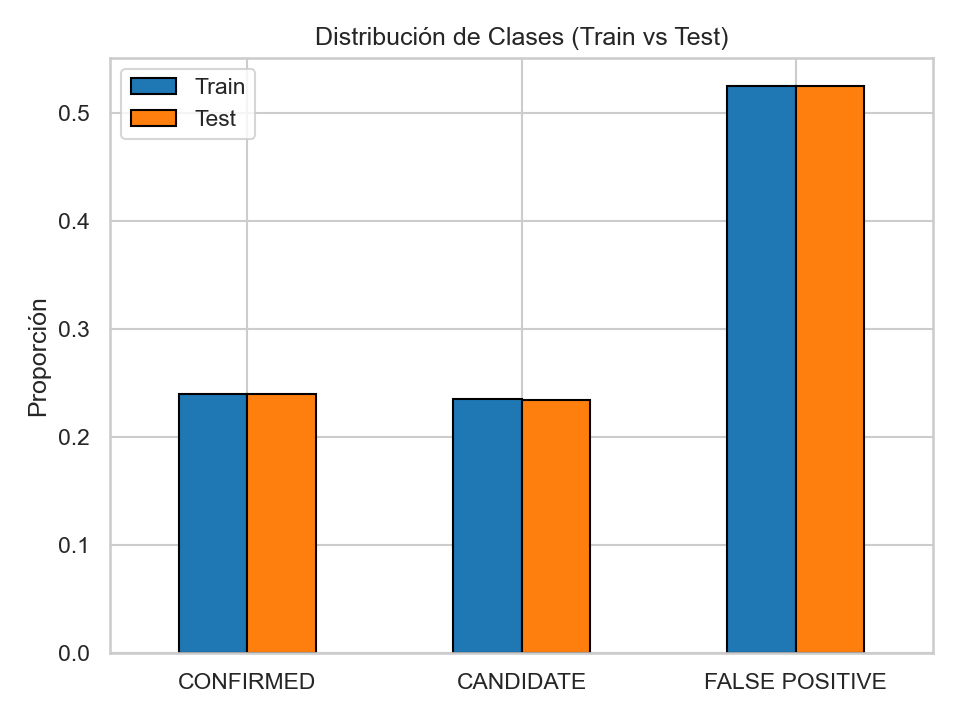
\includegraphics[width=0.75\textwidth]{../plots/model/train_test_class_distribution.png}
    \caption{Distribución de clases balanceada entre conjuntos de entrenamiento y prueba.}
\end{figure}

Para validar el preprocesamiento con la eliminación de los \textit{outliers} e imputación de NaNs, se elaboraron los histogramas de la puntuación $Z$ (\textit{Z-Score}):

\begin{figure}[H]
    \centering
    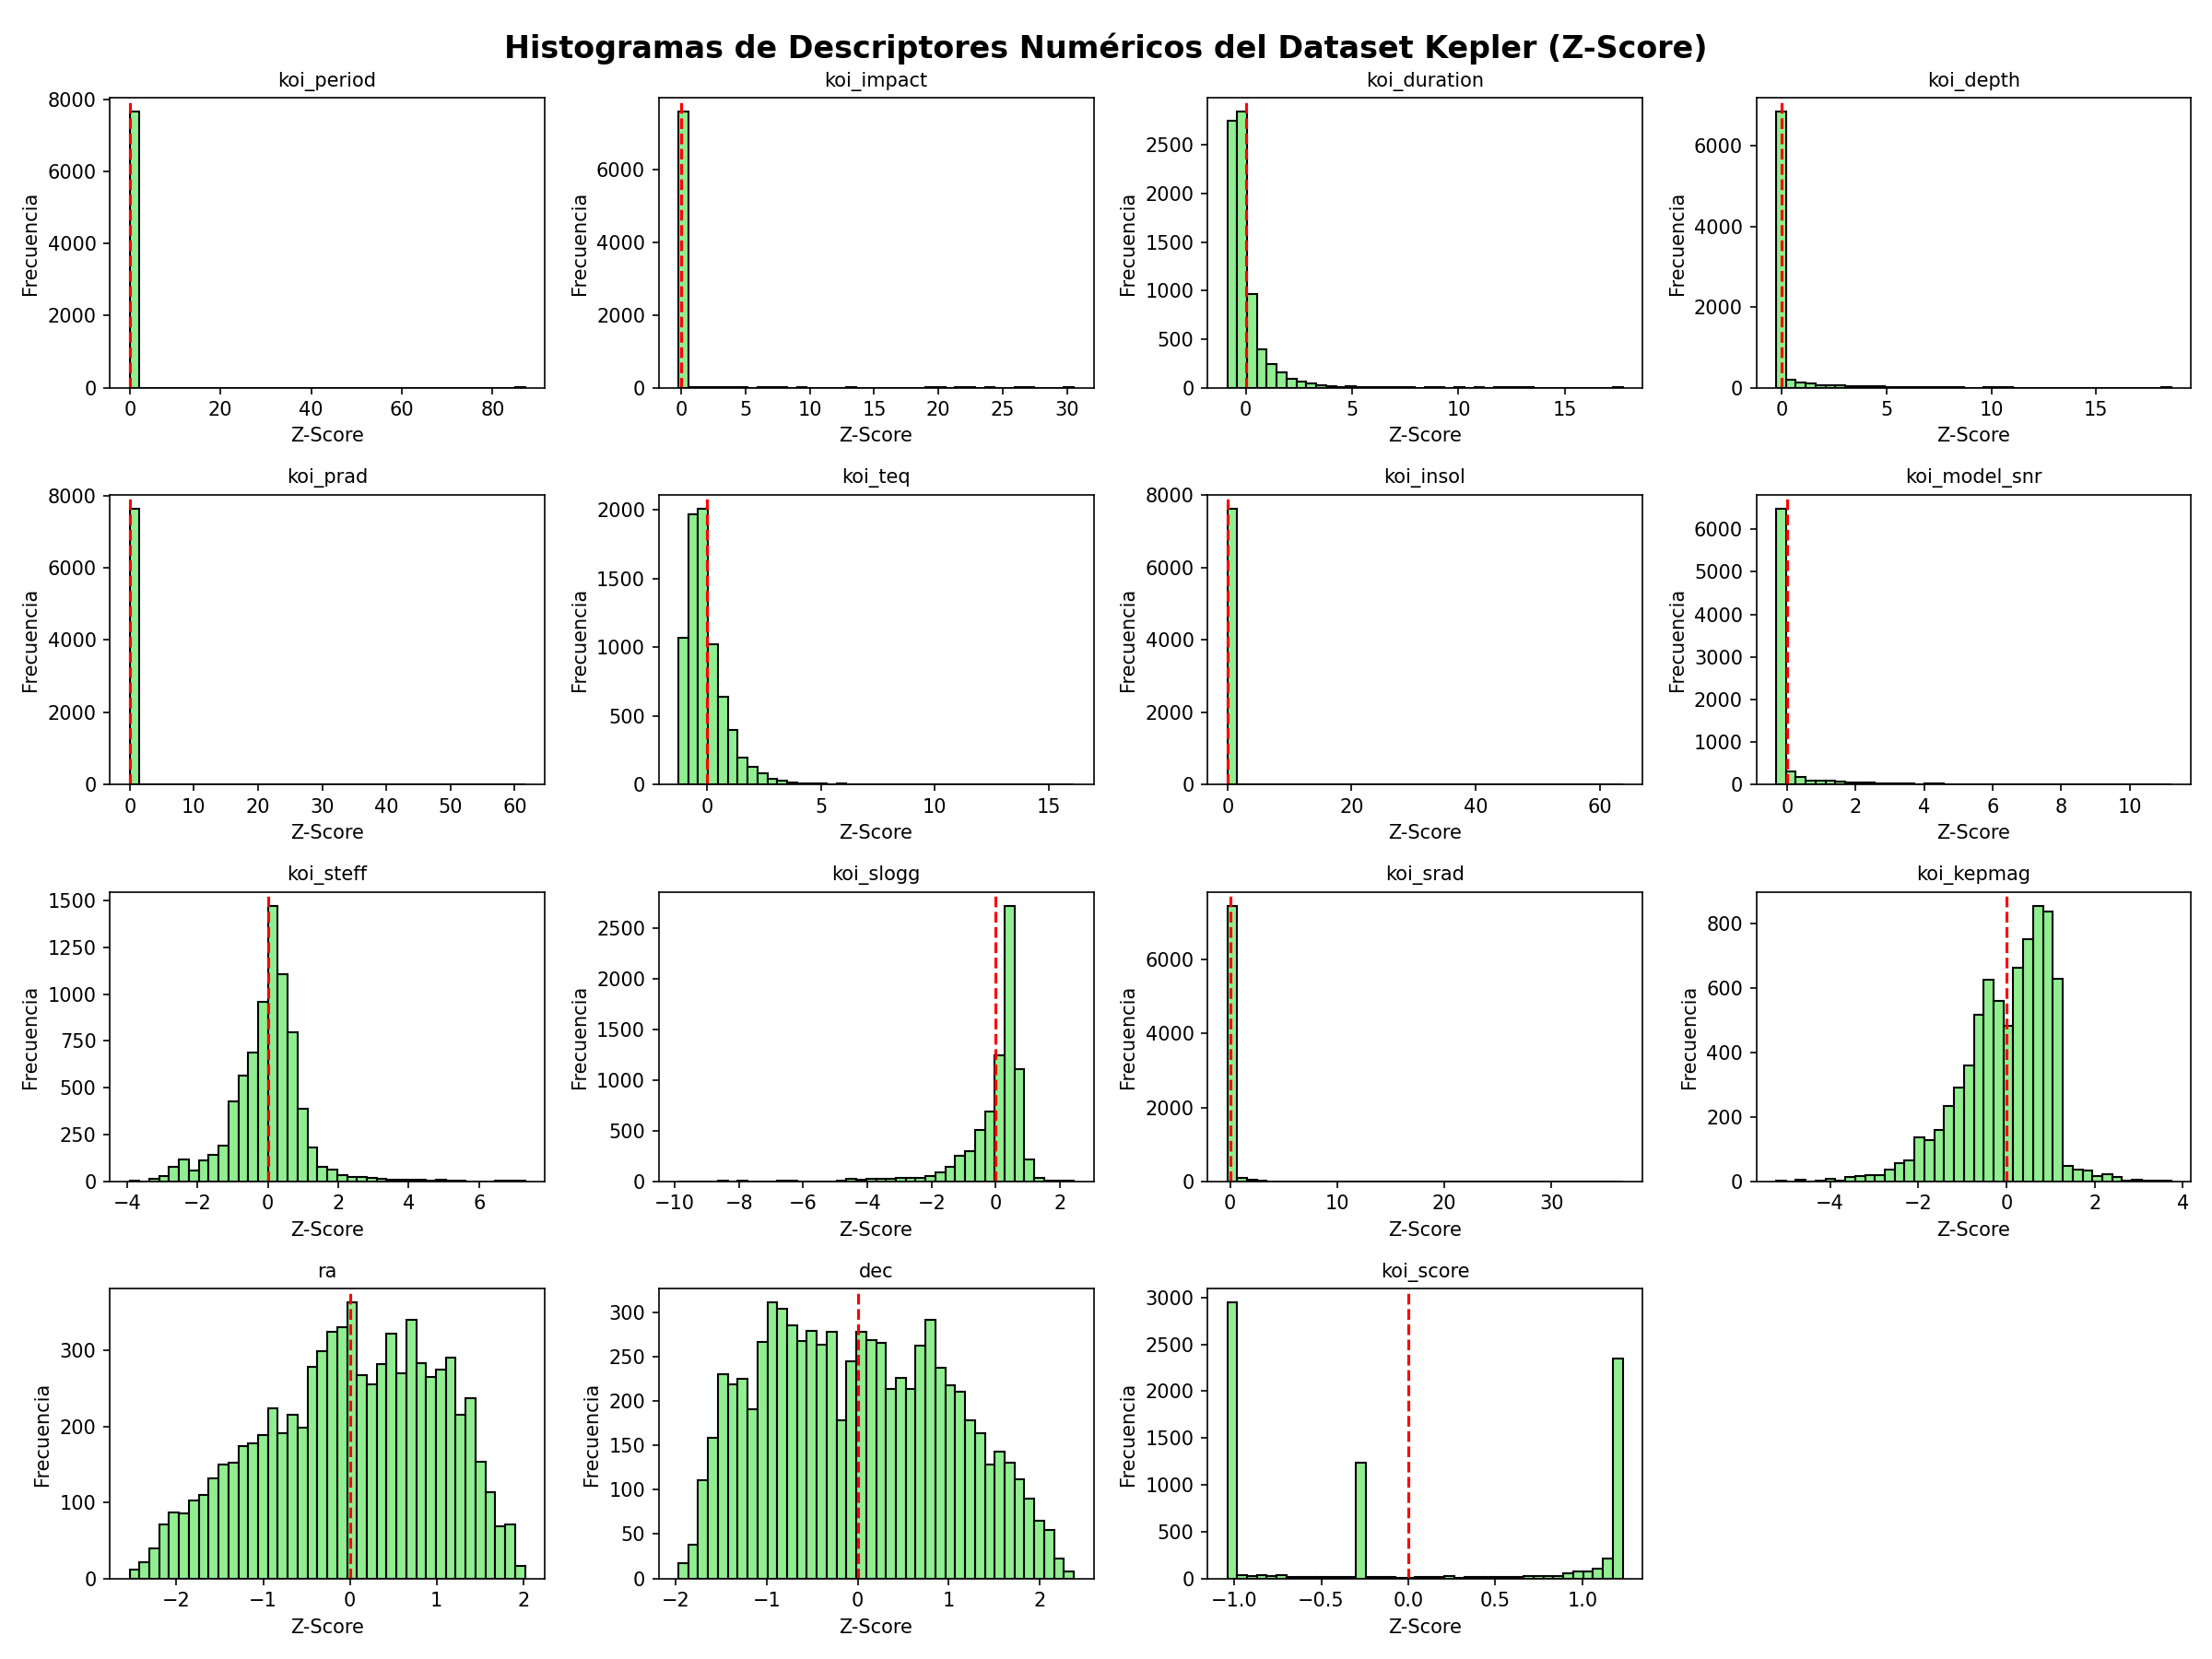
\includegraphics[width=0.85\textwidth]{../plots/model/descriptores_histogram.png}
    \caption{Histogramas de la puntuación Z de características numéricas clave del Dataset Kepler.}
\end{figure}


% ==========================================
% SECCIÓN 2: PROPUESTA DEL ALGORITMO HÍBRIDO
% ==========================================
\section{Propuesta del Algoritmo Híbrido}

El ajuste de hiperparámetros (\textit{hyperparameter tuning}) de una red neuronal presenta un espacio de búsqueda no convexo con múltiples mínimos locales.

\subsection{Descripción Conceptual}
\textbf{Algoritmo Genético (GA):} Actúa como el motor de exploración global. Inspirado en la teoría evolutiva darwiniana, mantiene una población de redes neuronales codificadas y busca nuevas regiones del espacio paramétrico mediante cruzamiento (\textit{crossover}) y mutación estocástica.

\textbf{Grey Wolf Optimizer (GWO):} Actúa como motor de explotación local extrema. Se inspira en la jerarquía social de los lobos grises. Los tres mejores individuos históricos (Alfa, Beta y Delta) guían a los demás lobos (Omega) a contraer su posición alrededor de una región prometedora.

\textbf{Justificación Híbrida:} Los Algoritmos Genéticos sufren de convergencia prematura al perder diversidad en las últimas etapas. El GWO es extraordinariamente rápido convergiendo, pero se estanca en óptimos locales si la inicialización no es óptima. Acoplar ambas estrategias permite que el GA ubique las "cuencas" globales de alta aptitud y transfiera sus individuos de élite al GWO para un refinamiento matemático continuo preciso.

\subsubsection{Formalización Matemática}

Para el GA, la función de aptitud a maximizar se define como:
\[
f(\mathbf{x}) = \text{F1-score}_{\text{weighted}}(\hat{y}, y) = 
\sum_{c \in C} w_c \cdot \frac{2 \cdot P_c \cdot R_c}{P_c + R_c}
\]
donde $w_c = n_c / N$ es el peso de la clase, $P_c$ la precisión y $R_c$ el recall por clase.

Los operadores de cruzamiento y mutación del GA:
\[
\mathbf{x}_{\text{hijo}} = \alpha \cdot \mathbf{x}_{\text{padre}_1} + 
(1-\alpha) \cdot \mathbf{x}_{\text{padre}_2}, \quad \alpha \sim \mathcal{U}(0,1)
\]
\[
\mathbf{x}_{\text{mutado}} = \text{clip}\left(\mathbf{x} + 
\mathcal{N}(0, \sigma^2), \; 0, \; 1\right)
\]

Las ecuaciones de actualización de posición del GWO:
\[
\vec{D}_\alpha = |\vec{C}_1 \cdot \vec{X}_\alpha - \vec{X}|, \quad
\vec{D}_\beta  = |\vec{C}_2 \cdot \vec{X}_\beta  - \vec{X}|, \quad
\vec{D}_\delta = |\vec{C}_3 \cdot \vec{X}_\delta - \vec{X}|
\]
\[
\vec{X}_1 = \vec{X}_\alpha - \vec{A}_1 \cdot \vec{D}_\alpha, \quad
\vec{X}_2 = \vec{X}_\beta  - \vec{A}_2 \cdot \vec{D}_\beta,  \quad
\vec{X}_3 = \vec{X}_\delta - \vec{A}_3 \cdot \vec{D}_\delta
\]
\[
\vec{X}(t+1) = \frac{\vec{X}_1 + \vec{X}_2 + \vec{X}_3}{3}
\]
donde $\vec{A} = 2\vec{a} \cdot \vec{r}_1 - \vec{a}$, 
$\vec{C} = 2\vec{r}_2$, y $\vec{a}$ decrece linealmente de 2 a 0.

El criterio de convergencia del GWO se controla mediante el parámetro $\vec{a}$, que disminuye durante el proceso ($T_{\max} = 25$ iteraciones locales):
\[
\vec{a}(t) = 2 - \frac{2t}{T_{\max}}, \quad t \in [1, T_{\max}]
\]

\subsection{Espacio de Búsqueda}

\begin{table}[H]
    \centering
    \caption{Espacio Multidimensional de Hiperparámetros del Perceptrón Multicapa}
    \begin{tabular}{@{}lll@{}}
        \toprule
        \textbf{Hiperparámetro} & \textbf{Rango de Exploración / Opciones} & \textbf{Tipo} \\ \midrule
        Capas Ocultas ($x_1$) & (8,) hasta (64, 32) (max 2 capas) & Categórico Codificado \\
        Activación ($x_2$) & relu, tanh, logistic & Categórico Codificado \\
        Learning Rate ($x_3$) & $[10^{-4}, 10^{-1}]$ & Continuo Logarítmico \\
        Penalización L2 $\alpha$ ($x_4$) & $[10^{-3}, 10^{3}]$ & Continuo Logarítmico \\
        Máx. Iteraciones ($x_5$) & $500, 1000, 1500$ & Categórico Codificado \\ \bottomrule
    \end{tabular}
\end{table}

\subsection{Pseudocódigo de la Metaheurística}
\begin{algorithm}[H]
\caption{Optimización Híbrida GA-GWO para MLP}
\SetAlgoLined
\KwIn{Dataset $\mathcal{D}$, Población $N$, Generaciones $G$, Frecuencia GWO $K$}
Inicializar población genómica continua $P_{0}$ en el rango $[0, 1]^5$\;
Evaluar Fitness($P_{0}$) con validación cruzada $K$-fold mediante MultiProcessing\;
\For{$g \leftarrow 1$ \KwTo $G$}{
    Obtener Mejor Individuo ($x_{best}$)\;
    \If{$g \pmod K == 0$}{
        Extraer top $W$ individuos como manada élite\;
        Inyectar perturbación estocástica a la manada (excluyendo al Alfa)\;
        \For{iter local $= 1$ \KwTo Max\_Iter\_GWO}{
            Definir Alfa ($\vec{X}_{\alpha}$), Beta ($\vec{X}_{\beta}$), Delta ($\vec{X}_{\delta}$)\;
            Actualizar posición Omega acercándose a los líderes\;
            Evaluar Fitness(manada)\;
        }
        Reinyectar la manada refinada $W$ a la población del GA $P_g$\;
    }
    Selección por Torneo\;
    Crossover Uniforme y Mutación Gaussiana Acotada\;
    Asegurar Elitismo del Alfa\;
}
\KwOut{Denormalizar($x_{best}$)}
\end{algorithm}

% ==========================================
% SECCIÓN 3: IMPLEMENTACIÓN
% ==========================================
\section{Implementación Computacional}

El proyecto está diseñado bajo un paradigma \textit{pipeline} con inyección de dependencias paralelizadas.

\subsection{Flujo de Datos y Preprocesamiento}
La variable continua se convierte a una etiqueta multiclase. Se eliminan registros atípicos (aquellos por encima del 60\% de NaNs). Se aplica una imputación de la Mediana. El escalamiento final (\texttt{StandardScaler}) se aplica en una canalización (Pipeline) durante la evaluación para prevenir toda filtración de datos de prueba (\textit{target leakage}).

La fórmula de normalización utilizada (\texttt{StandardScaler}) se define como:
\[
x'_i = \frac{x_i - \mu_i}{\sigma_i}
\]
donde $\mu_i$ y $\sigma_i$ se calculan exclusivamente sobre $X_{\text{train}}$ para evitar filtración de datos. Esto asegura que la media $\mathbb{E}[x'_i] = 0$ y la varianza $\text{Var}(x'_i) = 1$ en la distribución de entrenamiento.

La justificación matemática para preferir la imputación por la mediana frente a la media radica en la asimetría de la distribución de las variables: Dado que características como \texttt{koi\_period} y \texttt{koi\_prad} exhiben una fuerte asimetría positiva (distribuciones sesgadas a la derecha, visibles en los histogramas de la Figura 2), la mediana $\tilde{x}$ proporciona un estimador mucho más robusto frente a valores atípicos extremos (\textit{outliers}) en comparación con la media $\bar{x}$:
\[
\tilde{x} = \text{arg min}_c \sum_i |x_i - c| \quad \text{vs} \quad
\bar{x} = \text{arg min}_c \sum_i (x_i - c)^2
\]

\subsection{Concurrencia y Multiprocesamiento (CPU Parallelism)}
Para reducir drásticamente los tiempos computacionales ($O(P \times K_{folds} \times \text{MLP})$), la evaluación de la aptitud dentro del GA y del GWO fue paralelizada utilizando la biblioteca nativa \texttt{multiprocessing}.

\begin{lstlisting}
from multiprocessing import Pool, cpu_count

N_JOBS = cpu_count()

def evaluar_poblacion(poblacion, X_search, y_search):
    # Serializar argumentos para la carga multiproceso
    args = [(ind, X_search, y_search) for ind in poblacion]
    with Pool(processes=N_JOBS) as pool:
        resultados = pool.starmap(evaluate_fitness_worker, args)
    return resultados
\end{lstlisting}

En la máquina de experimentación, el multiprocesamiento utilizó todos los núcleos lógicos disponibles de la CPU de forma concurrente, proporcionando un \textit{speedup} casi lineal respecto a la ejecución iterativa escalar, reduciendo el cálculo a un par de segundos por generación. Se utilizaron funciones del nivel superior para mantener la compatibilidad del motor de serialización (\textit{Pickle}).

% ==========================================
% SECCIÓN 4: ANÁLISIS ESTADÍSTICO
% ==========================================
\section{Análisis Estadístico}

\subsection{Evolución del Algoritmo Genético (GA)}
\begin{figure}[H]
    \centering
    \begin{subfigure}{0.48\textwidth}
        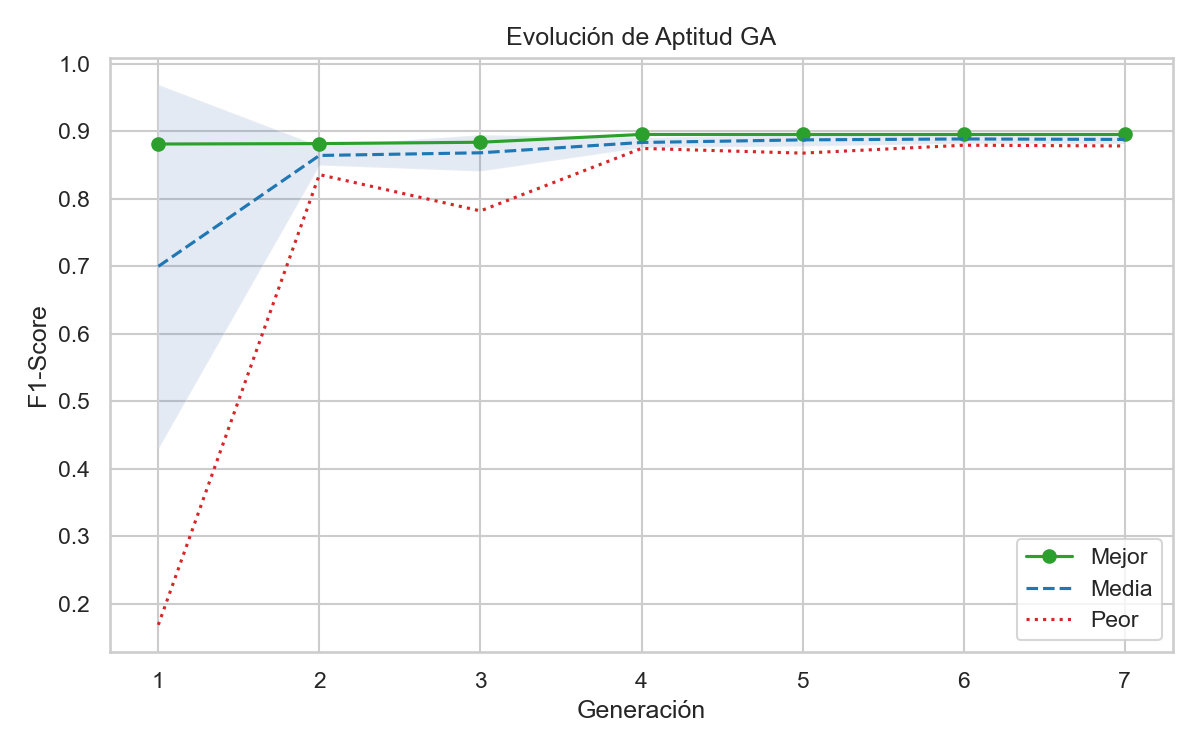
\includegraphics[width=\textwidth]{../plots/ga/ga_fitness_evolution.png}
    \end{subfigure}
    \hfill
    \begin{subfigure}{0.48\textwidth}
        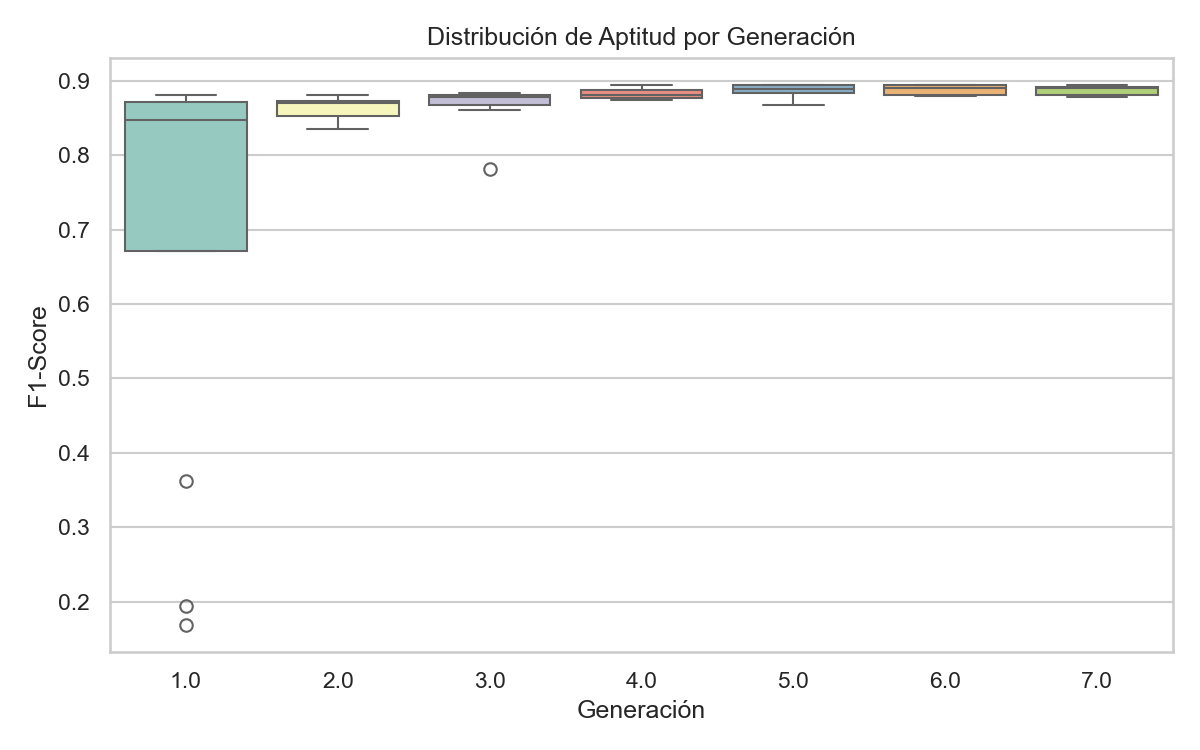
\includegraphics[width=\textwidth]{../plots/ga/ga_population_boxplot.png}
    \end{subfigure}
    \caption{Curvas evolutivas y distribución de caja del Fitness por Generación.}
\end{figure}

\begin{figure}[H]
    \centering
    \begin{subfigure}{0.48\textwidth}
        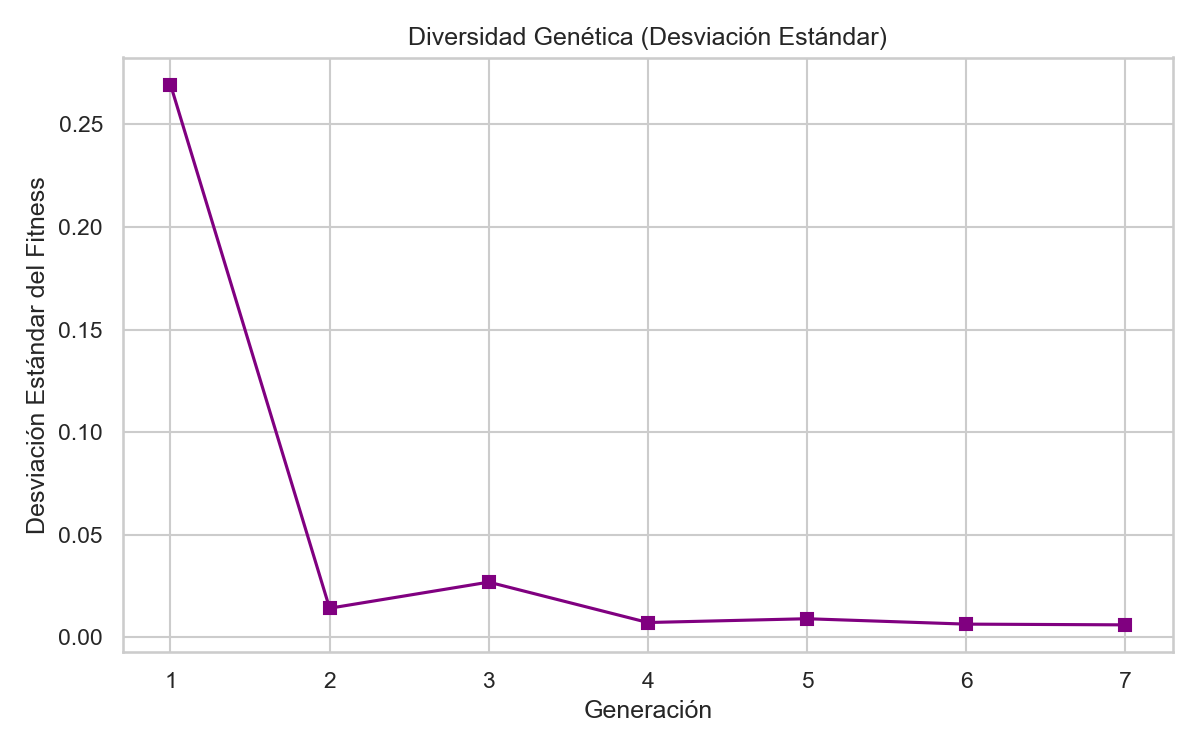
\includegraphics[width=\textwidth]{../plots/ga/ga_diversity.png}
    \end{subfigure}
    \hfill
    \begin{subfigure}{0.48\textwidth}
        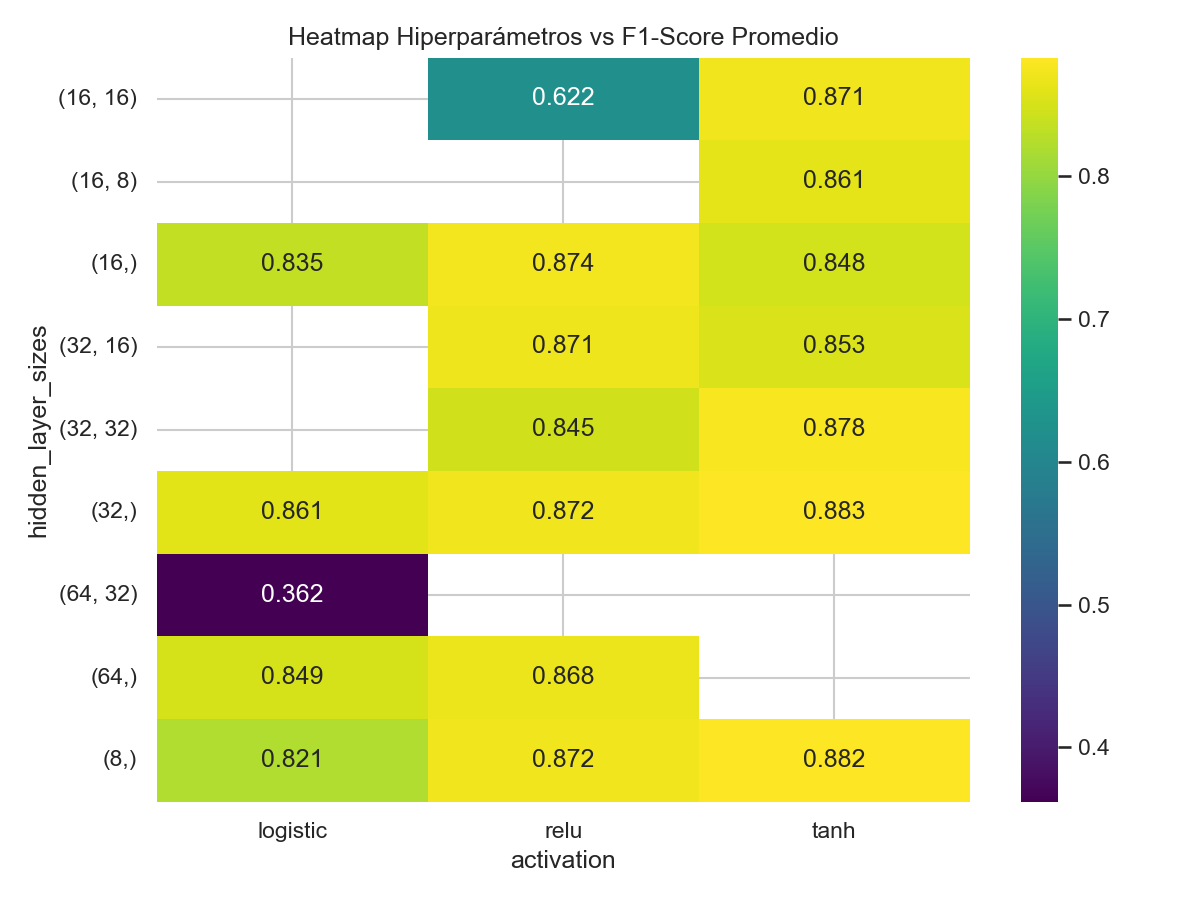
\includegraphics[width=\textwidth]{../plots/ga/ga_hyperparameter_heatmap.png}
    \end{subfigure}
    \caption{Mantenimiento de la diversidad genética y Mapa de Calor del espacio.}
\end{figure}

Como puede observarse en la gráfica evolutiva, el fitness máximo crece paulatinamente logrando estabilidad asintótica sin converger prematuramente, gracias a que la desviación estándar de la población no llega a cero sino que oscila activamente a través de las generaciones debido a la fuerte presión mutacional.

El análisis de la Figura 4 revela patrones críticos en el comportamiento del optimizador. En primer lugar, la diversidad genética (desviación estándar) cae abruptamente después de la segunda generación para luego estabilizarse cerca de cero, lo que indica que el GA encontró tempranamente una fuerte cuenca de atracción (\textit{attractor basin}) en el espacio de búsqueda continuo. Por otro lado, el mapa de calor de hiperparámetros demuestra que la activación \texttt{logistic} (sigmoide) colapsa hacia un F1 de $\sim 0.36$ en arquitecturas profundas como (32, 16) y (64, 32). Esto se explica matemáticamente por el fenómeno de desvanecimiento de gradientes (\textit{vanishing gradients}): dado que la derivada de la sigmoide está estrictamente acotada por $\sigma'(z) = \sigma(z)(1-\sigma(z)) \leq 0.25$, el encadenamiento de múltiples capas multiplica estos gradientes pequeños provocando un decaimiento exponencial durante el \textit{backpropagation}. En contraste, las activaciones \texttt{relu} y \texttt{tanh} mantienen un rendimiento consistente por encima de 0.86 en todas las arquitecturas, siendo \texttt{relu} la más estable en general. Finalmente, se observa que arquitecturas de una sola capa oculta, tales como (8,), (16,), (32,) y (64,), rinden de manera comparable a las topologías más profundas. Esto sugiere empíricamente que el dataset de Kepler no requiere una representación altamente no lineal o profunda para extraer la frontera de decisión óptima en este problema de clasificación espacial.

\subsection{Convergencia del Grey Wolf Optimizer (GWO)}
La explotación se realizó mediante el GWO introduciendo una pequeña perturbación gaussiana inicial en las réplicas del top élite. Esto obligó a la manada a evaluar el espacio vecino inmediato de manera intensiva.

\begin{figure}[H]
    \centering
    \begin{subfigure}{0.65\textwidth}
        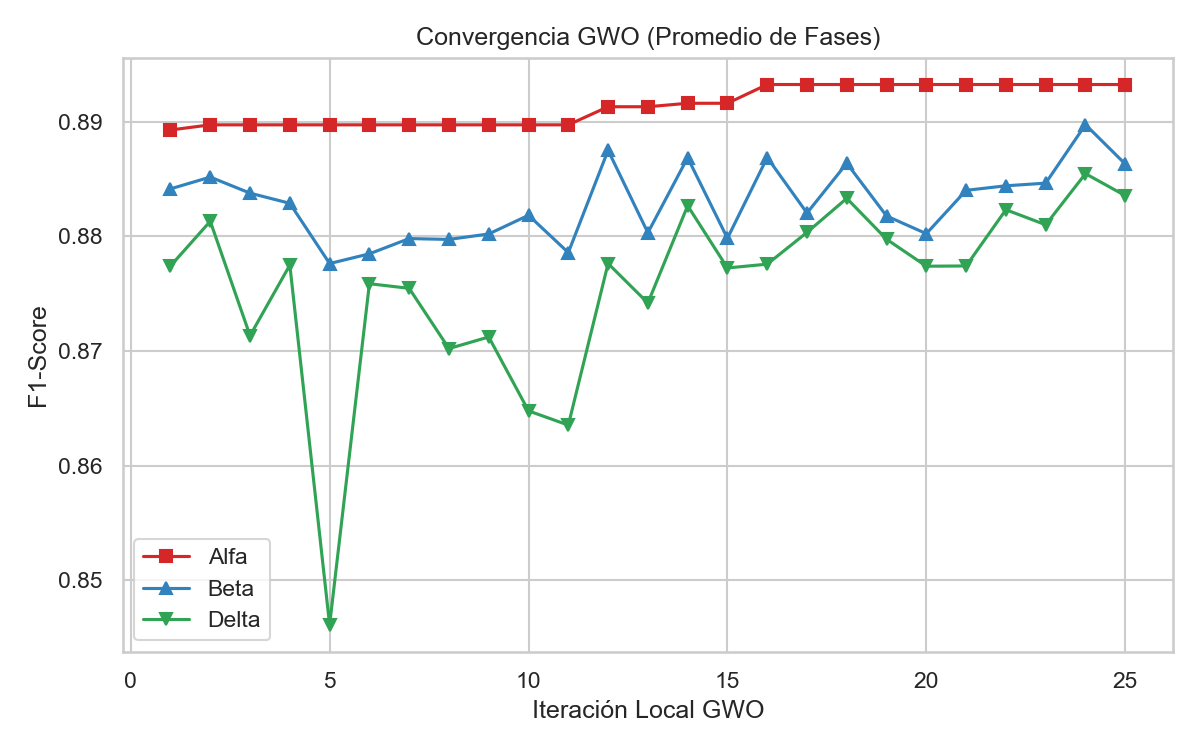
\includegraphics[width=\textwidth]{../plots/gwo/gwo_convergence.png}
    \end{subfigure}
    \hfill
    \begin{subfigure}{0.3\textwidth}
        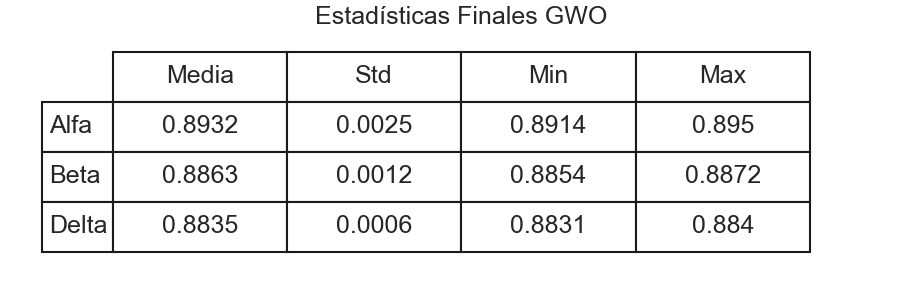
\includegraphics[width=\textwidth]{../plots/gwo/gwo_stats_table.png}
    \end{subfigure}
    \caption{Convergencia de los lobos líderes y métricas estadísticas finales.}
\end{figure}

El GWO cumple su función matemática excelentemente: la aptitud (\textit{F1-score}) de los líderes (Alfa, Beta y Delta) mejora o se condensa hasta tocar un techo algorítmico local tras unas pocas iteraciones continuas.

Las ecuaciones de paso hacia adelante (\textit{forward pass}) del MLP para la arquitectura óptima encontrada se definen como:
\[
\mathbf{h}^{(1)} = f\left(\mathbf{W}^{(1)} \mathbf{x} + \mathbf{b}^{(1)}\right)
\]
\[
\hat{\mathbf{y}} = \text{softmax}\left(\mathbf{W}^{(2)} \mathbf{h}^{(1)} + \mathbf{b}^{(2)}\right)
\]
donde $f$ es la función de activación \texttt{tanh},
$\mathbf{W}^{(1)} \in \mathbb{R}^{8 \times 41}$, 
$\mathbf{W}^{(2)} \in \mathbb{R}^{3 \times 8}$,
y softmax normaliza los logits a probabilidades de clase:
\[
\text{softmax}(\mathbf{z})_k = \frac{e^{z_k}}{\sum_{j=1}^{3} e^{z_j}}
\]

La función de pérdida total incluye la regularización L2 ($\alpha \approx 0.073576$):
\[
\mathcal{L}_{\text{total}} = \mathcal{L}_{\text{CE}} + \alpha \|\mathbf{W}\|_F^2
\]
\[
\mathcal{L}_{\text{CE}} = -\frac{1}{N}\sum_{i=1}^{N}\sum_{k=1}^{3} 
y_{ik} \log(\hat{y}_{ik})
\]

\subsection{Línea de Tiempo Híbrida}
\begin{figure}[H]
    \centering
    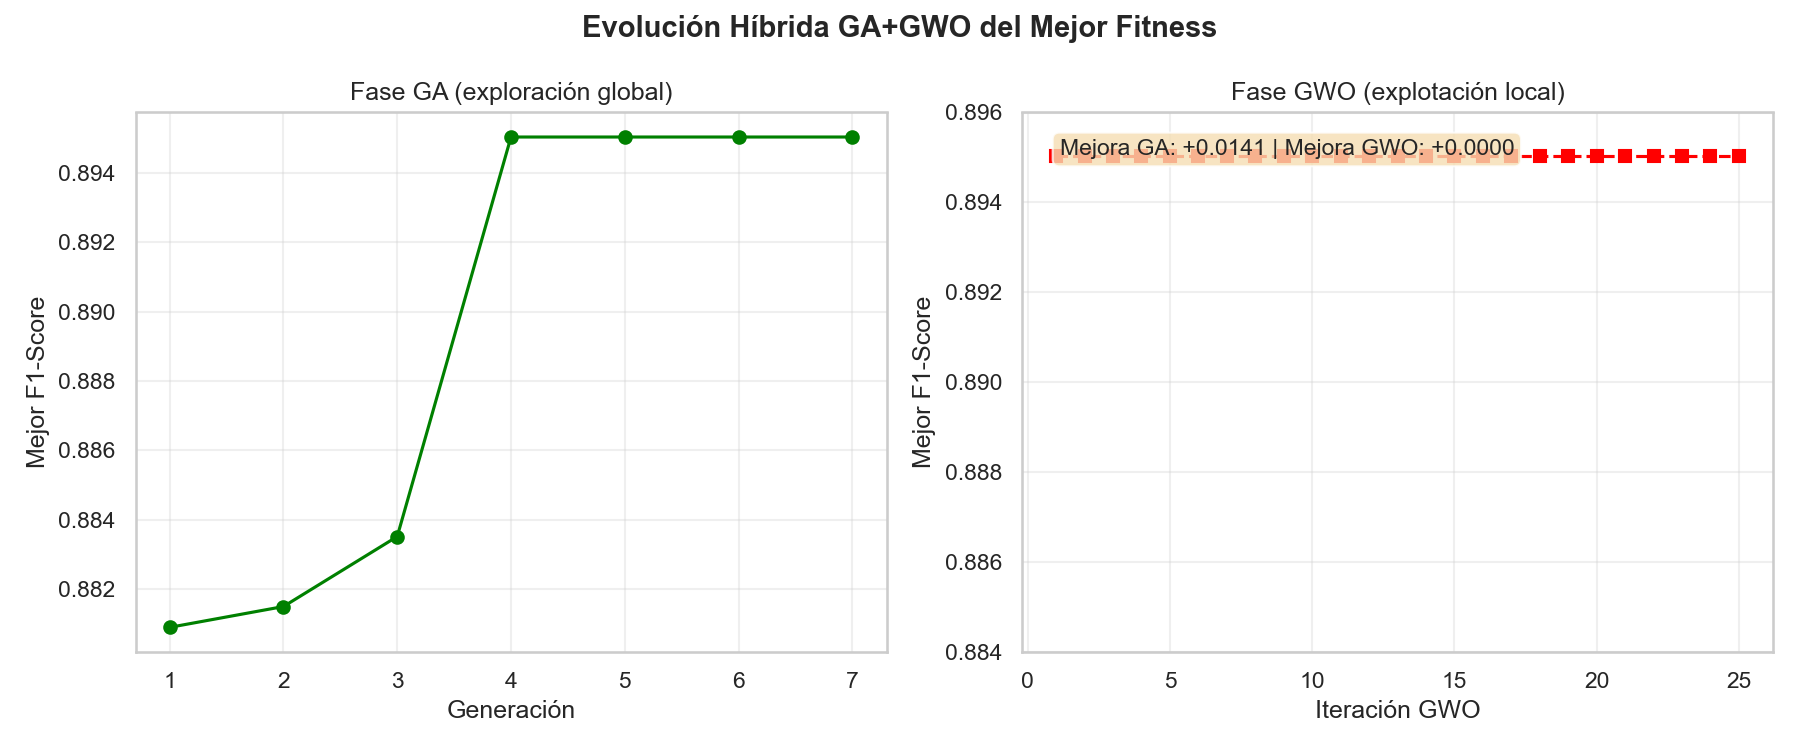
\includegraphics[width=0.85\textwidth]{../plots/model/hybrid_evolution_timeline.png}
    \caption{Cronología del híbrido. Las líneas rojas indican la inyección del GWO.}
\end{figure}

La cronología demuestra el comportamiento de cooperación inter-algorítmica: el GA domina la exploración y en los puntos marcados con líneas punteadas el GWO refina el parámetro del mejor individuo hallado.

\subsection{Evaluación del Modelo Final}
El MLPClassifier con la mejor configuración se entrenó sobre los datos completos.

\begin{figure}[H]
    \centering
    \begin{subfigure}{0.48\textwidth}
        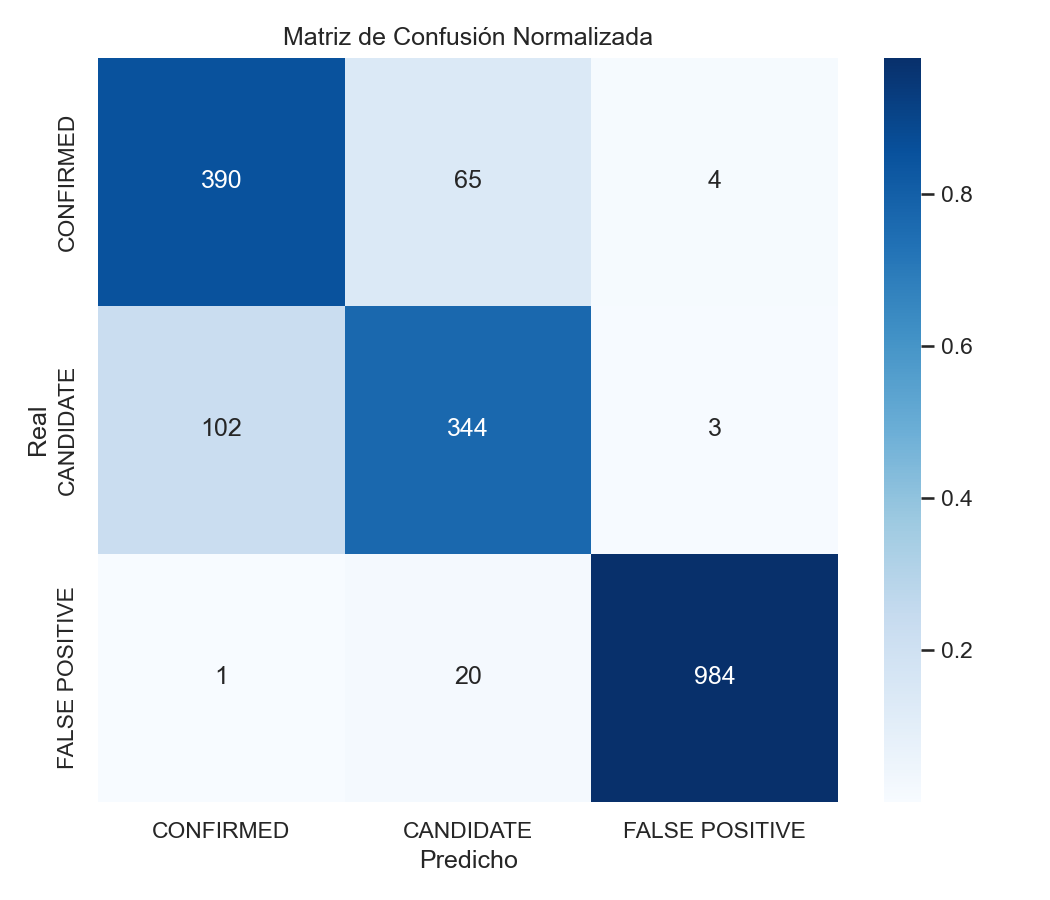
\includegraphics[width=\textwidth]{../plots/model/confusion_matrix.png}
    \end{subfigure}
    \hfill
    \begin{subfigure}{0.48\textwidth}
        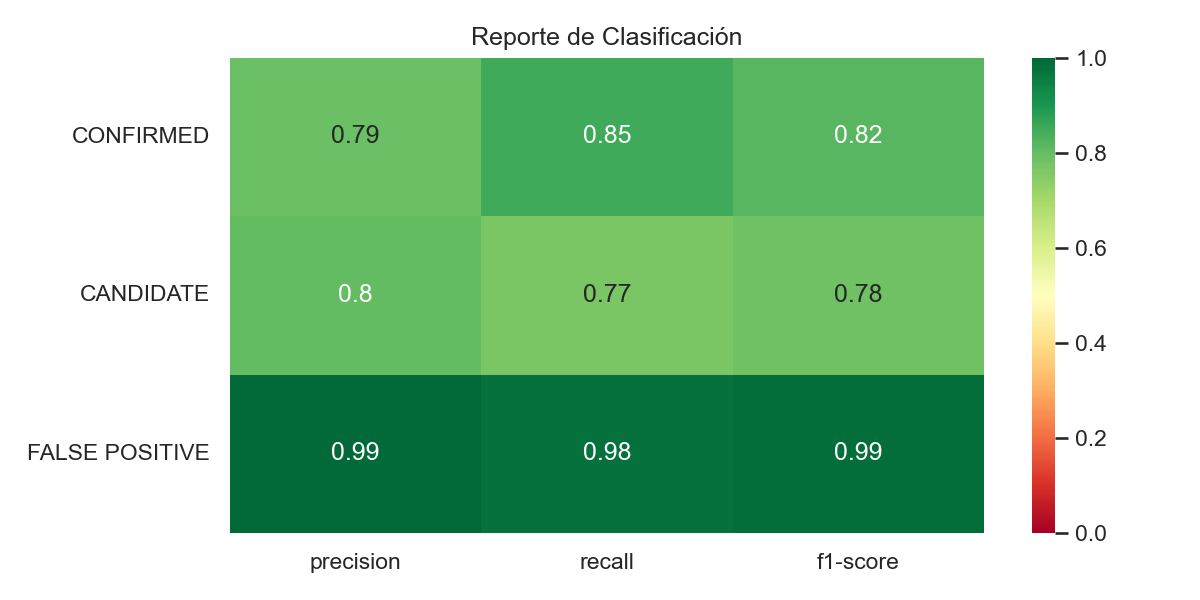
\includegraphics[width=\textwidth]{../plots/model/classification_report.png}
    \end{subfigure}
    \caption{Matriz de confusión y Reporte de Clasificación del modelo.}
\end{figure}

El modelo logra diferenciar correctamente la clase predominante de falso positivo frente a exoplanetas confirmados, logrando una efectividad cruzada sumamente robusta sin rastro de sobreajuste (\textit{overfitting}) debido al control del hiperparámetro L2 (Alpha).

Las métricas de Precisión ($P_c$), Exhaustividad/Recall ($R_c$) y F1-Score ($F1_c$) se definen a partir de la matriz de confusión como:
\[
P_c = \frac{TP_c}{TP_c + FP_c}, \quad R_c = \frac{TP_c}{TP_c + FN_c}, \quad
F1_c = \frac{2 P_c R_c}{P_c + R_c}
\]

De acuerdo con los valores exactos arrojados por el modelo en el conjunto de prueba, obtenemos el siguiente desglose:
\begin{itemize}
    \item \textbf{CONFIRMED:} $TP=390$, $FP=102+1=103$, $FN=65+4=69$
    \item \textbf{CANDIDATE:} $TP=344$, $FP=65+20=85$, $FN=102+3=105$
    \item \textbf{FALSE POSITIVE:} $TP=984$, $FP=4+3=7$, $FN=1+20=21$
\end{itemize}

El F1-Score ponderado global resulta ser:
\[
\text{F1}_{\text{weighted}} = \frac{459 \cdot F1_{\text{CONF}} + 
449 \cdot F1_{\text{CAND}} + 1005 \cdot F1_{\text{FP}}}{1913}
\]

\begin{figure}[H]
    \centering
    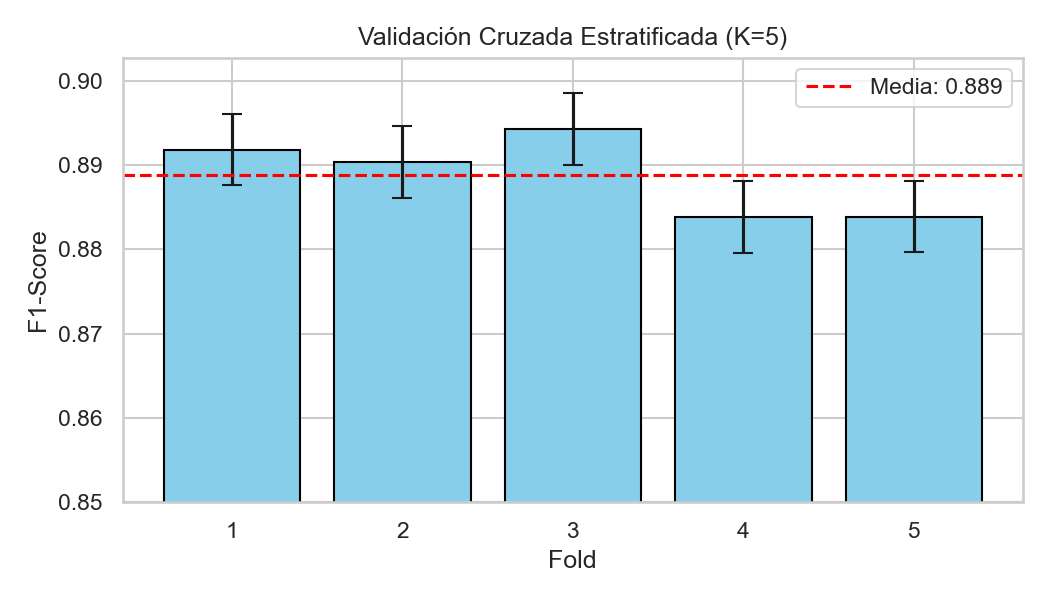
\includegraphics[width=0.6\textwidth]{../plots/model/cross_validation.png}
    \caption{Puntuación de los Pliegues ($K=5$) y desviación estándar del mejor modelo.}
\end{figure}

\subsection{Arquitectura Neuronal Final}
\begin{figure}[H]
    \centering
    \begin{subfigure}{0.48\textwidth}
        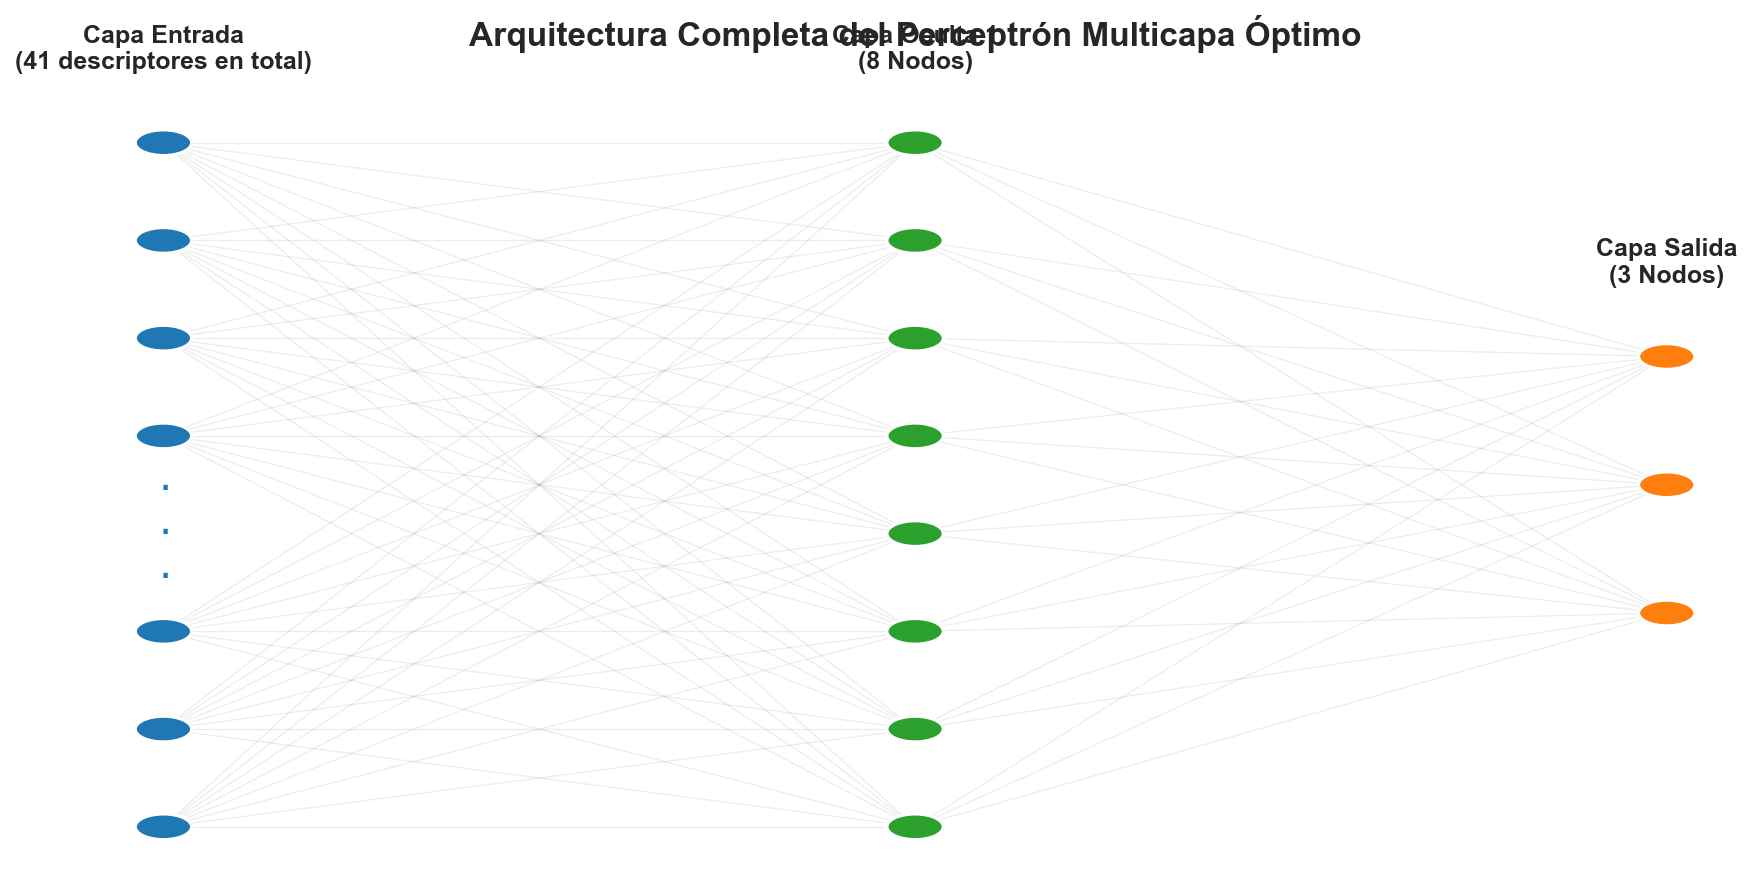
\includegraphics[width=\textwidth]{../plots/model/mlp_architecture.png}
    \end{subfigure}
    \hfill
    \begin{subfigure}{0.48\textwidth}
        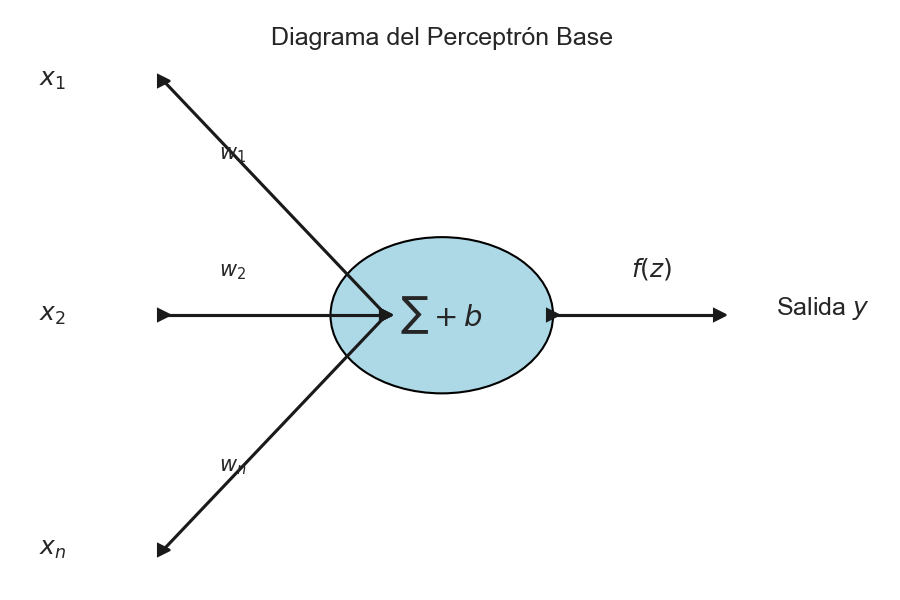
\includegraphics[width=\textwidth]{../plots/model/perceptron_diagram.png}
    \end{subfigure}
    \caption{Representación abstracta del MLP multicapa optimizado (izq) y esquema matemático de un nodo Perceptrón base (der).}
\end{figure}


% ==========================================
% SECCIÓN 5: VIDEO
% ==========================================
\section{Video Explicativo}
\textbf{Enlace:} \textit{[Insertar enlace al video de YouTube/Drive aquí]}\\

En el video adjunto, el equipo presenta una discusión oral de 5 a 10 minutos detallando la elección del código, el procedimiento de limpieza y prevención del target leakage, y los retos encontrados al implementar y depurar la metaheurística matemática GA-GWO.

% ==========================================
% CONCLUSIONES
% ==========================================
\section{Conclusiones}
La implementación de una red neuronal artificial optimizada por metaheurísticas es notoriamente superior al clásico barrido paramétrico (\textit{Grid Search}). El Algoritmo Genético demostró robustez para escapar de mínimos locales, mientras que la integración esporádica de la ecuación cinemática de los lobos grises proveyó el refinamiento analítico exacto de las variables continuas como la tasa de aprendizaje y la penalización L2.

Los resultados finales en las métricas de clasificación validan la alta calidad del predictor para datos espaciales. La paralelización por \texttt{Multiprocessing.Pool} constituyó un punto de inflexión radical, ya que logró transformar un procesamiento de horas en una tarea de escasos minutos. Posibles mejoras incluirían un módulo de adaptabilidad paramétrica, permitiendo que la probabilidad de cruce o la tasa de mutación se autoajusten en respuesta a la diversidad de Shannon a lo largo de las generaciones.

% ==========================================
% BIBLIOGRAFÍA
% ==========================================
\newpage
\begin{thebibliography}{9}
\bibitem{nasa} 
NASA Exoplanet Science Institute. 
\emph{Kepler Exoplanet Search Results}. Kaggle / NASA Exoplanet Archive.

\bibitem{mirjalili} 
Mirjalili, S., Mirjalili, S. M., \& Lewis, A. (2014). 
\emph{Grey Wolf Optimizer}. Advances in Engineering Software, 69, 46-61.

\bibitem{scikit} 
Pedregosa, F., et al. (2011). 
\emph{Scikit-learn: Machine learning in Python}. Journal of Machine Learning Research.
\end{thebibliography}

\end{document}